\documentclass[11pt, dvipdfmx]{beamer}
%\documentclass[8,9,10,11,12,14,17,20pt, dvips, handout]{beamer}
%%%%%%%%%%%  package  %%%%%%%%%%%
\usepackage{amssymb,amsmath,ascmac}
\usepackage{atbegshi}

\AtBeginShipoutFirst{\special{pdf:tounicode 90ms-RKSJ-UCS2}}
\usepackage{minijs}
\renewcommand{\kanjifamilydefault}{\gtdefault}
\usepackage{multirow}
\usepackage{bm}

\usepackage{tikz}
\usepackage{xparse}
\usetikzlibrary{shapes,arrows}
%% define fancy arrow. \tikzfancyarrow[<option>]{<text>}. ex: \tikzfancyarrow[fill=red!5]{hoge}
  \tikzset{arrowstyle/.style n args={2}{inner ysep=0.1ex, inner xsep=0.5em, minimum height=2em, draw=#2, fill=black!20, font=\sffamily\bfseries, single arrow, single arrow head extend=0.4em, #1,}}
  \NewDocumentCommand{\tikzfancyarrow}{O{fill=black!20} O{none}  m}{
    \tikz[baseline=-0.5ex]\node [arrowstyle={#1}{#2}] {#3 \mathstrut};}

%微分関連のマクロ
%
\newcommand{\diff}{\mathrm d}
\newcommand{\difd}[2]{\dfrac{\diff #1}{\diff #2}}
\newcommand{\difp}[2]{\dfrac{\partial #1}{\partial #2}}
\newcommand{\difdd}[2]{\dfrac{\diff^2 #1}{\diff #2^2}}
\newcommand{\difpp}[2]{\dfrac{\partial^2 #1}{\partial #2^2}}

\renewcommand\appendixname{Appendix}

%%%%%%%%%%%  theme  %%%%%%%%%%%

%%%%%
% Simple
%%%%%
%\usetheme{default}
%\usetheme{Pittsburgh}
%\usetheme{Rochester}
%\usetheme{Szeged}

%%%%%
% So So
%%%%%
%\usetheme{Singapore}
%\usetheme{CambridgeUS}
\usetheme{Copenhagen}
%\usetheme{Luebeck}
%\usetheme{Malmoe}
%\usetheme{Warsaw}

%%%%%
% No Heasder
%%%%%
%\usetheme{Madrid}
%\usetheme{Boadilla}

%%%%%
% No Footer
%%%%%
%\usetheme{Darmstadt}
%\usetheme{JuanLesPins}
%\usetheme{Montpellier}

%%%%%
% Color
%%%%%
%\usetheme{AnnArbor}

%%%%%
% Too much
%%%%%
%\usetheme{Berlin}
%\usetheme{Ilmenau}

%%%%%
% Right hand Side
%%%%%
%\usetheme{Goettingen}
%\usetheme{Marburg}

%%%%%
% Left hand Side
%%%%%
%\usetheme{PaloAlto}


%%%%%%%%%%%  inner theme  %%%%%%%%%%%
\useinnertheme{default}
%\useinnertheme{circles}
%\useinnertheme{inmargin}
%\useinnertheme{rectangles}
%\useinnertheme{rounded}


%%%%%%%%%%%  outer theme  %%%%%%%%%%%
\useoutertheme{default}
%\useoutertheme{miniframes}
%\useoutertheme{infolines}
%\useoutertheme{miniframes}
%\useoutertheme{smoothbars}
%\useoutertheme{sidebars}
%\useoutertheme{split}
%\useoutertheme{shadow}
%\useoutertheme{tree}
%\useoutertheme{smoothtree}


%%%%%%%%%%%  color theme  %%%%%%%%%%%
%\usecolortheme{structure}
%\usecolortheme{sidebartab}
%\usecolortheme{albatross}
%\usecolortheme{beetle}
%\usecolortheme{dove}
%\usecolortheme{crane}
%\usecolortheme{fly}
%\usecolortheme{seagull}
%\usecolortheme{wolverine}
%\usecolortheme{beaver}
%\usecolortheme{lily}
%\usecolortheme{orchid}
%\usecolortheme{rose}
%\usecolortheme{whale}
%\usecolortheme{seahorse}
%\usecolortheme{dolphin}


%%%%%%%%%%%  font theme  %%%%%%%%%%%
\usefonttheme{professionalfonts}
%\usefonttheme{default}
%\usefonttheme{serif}
%\usefonttheme{structurebold}
%\usefonttheme{structureserif}
%\usefonttheme{structuresmallcapsserif}


%%%%%%%%%%%  degree of transparency  %%%%%%%%%%%
%\setbeamercovered{transparent=30}

%\setbeamercolor{item}{fg=red}
\setbeamertemplate{items}[default]

%%%%%%%%%%%  numbering  %%%%%%%%%%%
%\setbeamertemplate{numbered}

\setbeamertemplate{navigation symbols}{}
%%%%%%%%%%%%%%%%%%%%%%%%%%%%%%%%%%%
\title
[MD シミュレーションによるネットワークポリマーのゴム弾性]
{MD シミュレーションによる\\ネットワークポリマーのゴム弾性}
\author[東亞合成 佐々木]{佐々木裕}
\institute[東亞合成]{東亞合成}
\date{December 19, 2019}
%%%%%%%%%%%%%%%%%%%%%%%%%%%%%%%%%%
\begin{document}
%%%%%%%%%%%%%%%%%%%%%%%%%%%%%%%%%%
\begin{frame}\frametitle{}
	\titlepage
\end{frame}
%%%%%%%%%%%%%%%%%%%%%
\section*{}
%
\begin{frame}
%[allowframebreaks]
{Outline}
	\tableofcontents
\end{frame}
%%%%%%%%%%%%%%%%%%%%%
\section{はじめに}
%%%%%%%%%%%%%%%%%
%%%%%%%%%%%%%%%%%%%%%%%%%%%%%%%%%%%%%%%%%%%%%
\subsection{本研究の目標とアプローチ}
%%%%%%%%%%%%%%%%%%%%%%%%%%%
%%%%%%%%%%%%%%%%%%%%%%%%%%%
\begin{frame}
\frametitle{本研究の目標とアプローチ}
\vspace{-2mm}
\begin{exampleblock}{本研究の目標とアプローチ}
\begin{itemize}
\item
目標\\
破壊耐性に優れた軽量材料の設計指針を明確化
\item
アプローチ
	\begin{itemize}
	\item
	可逆性に優れた材料としてゴム材料を選択。
	\item
	構造明確なネットワークの構築のために超分子ネットワーク。
	\item
	既知のモデルとの\color{red}多数の整合点と、興味深い不整合\color{black}を確認。
	\item
	\color{red}シミュレーションでマルチスケールモデル\color{black}を構築したい。
	\end{itemize}
\end{itemize}
\end{exampleblock}
\vspace{-2mm}
\begin{alertblock}{シミュレーションでやりたいこと}
\begin{itemize}
\item
できるだけ\alert{単純化したモデルで小さなスケール}から始めたい。
\item
まずは、長さの揃ったストランドで MD シミュレーション
\item
最終的に、亀裂先端の挙動を FEM シミュレーション
\end{itemize}
\centering
{\color{red}\Large「オッカムの剃刀」}
\end{alertblock}
\end{frame}
%%%%%%%%%%%%%%%%%%%%%%%%%%%%%%%%%%%%%%%%%%%%%
\subsection{規則ネットワーク構造での検討結果}
%%%%%%%%%%%%%%%%%%%%%%%%%%%
\begin{frame}
\frametitle{これまでのMDシミュレーション}
\begin{columns}[totalwidth=1\textwidth]
\column{.49\textwidth}
ストランド長を一定とした\\規則構造
\begin{itemize}
 \item 
 分岐数 
 	\begin{itemize}
 	\item  
 	三分岐\\
 	K4 構造
 	\item
 	四分岐\\
 	ダイヤモンド構造
	\end{itemize}
 \item 
 ストランド
 	\begin{itemize}
 	\item  
 	KG鎖\\
 	LJ ポテンシャルにより、排除体積効果を導入
 	\item
	素抜け鎖\\
	長距離相互作用を無視した理想鎖
	\end{itemize}
\end{itemize}
\column{.49\textwidth}
K4 構造
\vspace{-3mm}
\begin{figure}
\centering
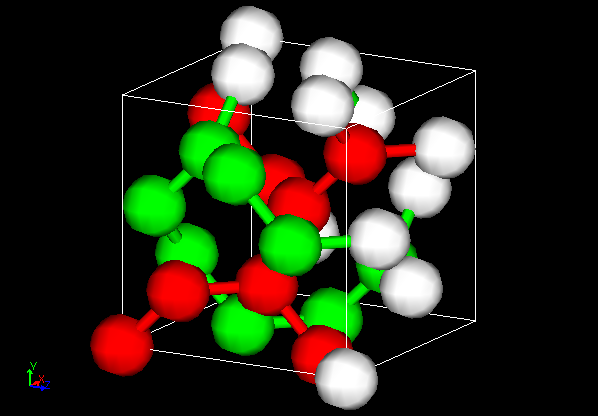
\includegraphics[width=0.7\textwidth]{./fig/K4_d.png}
\end{figure}
ダイヤモンド構造
\vspace{-3mm}
\begin{figure}
\centering
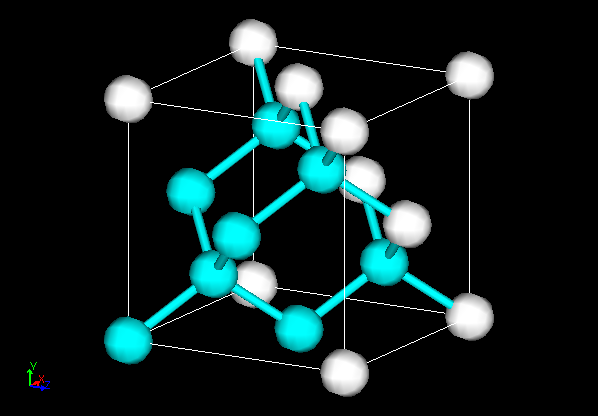
\includegraphics[width=0.7\textwidth]{./fig/dia.png}
\end{figure}
\end{columns}
\end{frame}
%%%%%%%%%%%%%%%%%%%%%%%%%%%%%%%%%%%%%%
\begin{frame}
\frametitle{規則ネットワーク構造での検討結果}

\vspace{-2mm}
\small
\begin{alertblock}{規則ネットワーク構造の振る舞い}
\begin{itemize}
\item
一軸伸長結果
	\begin{itemize}
	\item
	\alert{アフィンネットワークモデルの挙動}を示した\\\alert{分岐数、ストランドの性質によらず}(KGでも素抜けでも)
%	\item
%	伸びきり効果をほぼ再現
	\end{itemize}
\item
応力緩和挙動から、主緩和が\alert{ラウスモードの最長緩和時間程度}
\item
主緩和近傍に\alert{大きなエネルギー散逸($\tan \delta > 1$)}を確認
\end{itemize}
\end{alertblock}

\begin{columns}[totalwidth=1\textwidth]
\column{.32\textwidth}
\scriptsize
一軸伸長結果
\vspace{-2mm}
\begin{figure}
\centering
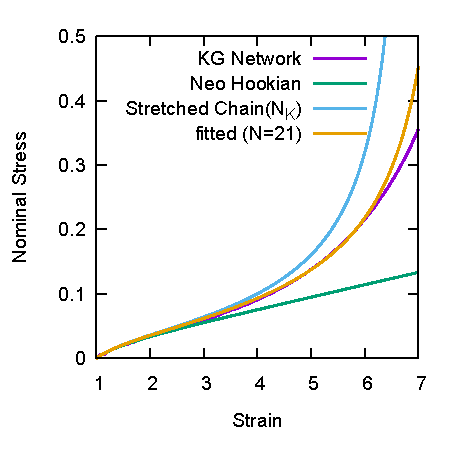
\includegraphics[width=0.9\textwidth]{./fig/SS_Kuhn.pdf}
\end{figure}
\column{.32\textwidth}
\scriptsize
応力緩和挙動
\vspace{-2mm}
\begin{figure}
\centering
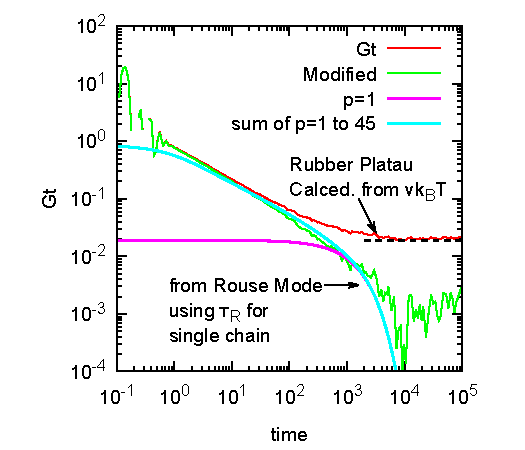
\includegraphics[width=0.9\textwidth]{./fig/Gt_loglog.pdf}
\end{figure}
\column{.32\textwidth}
\scriptsize
粘弾性スペクトル
\vspace{-2mm}
\begin{figure}
\centering
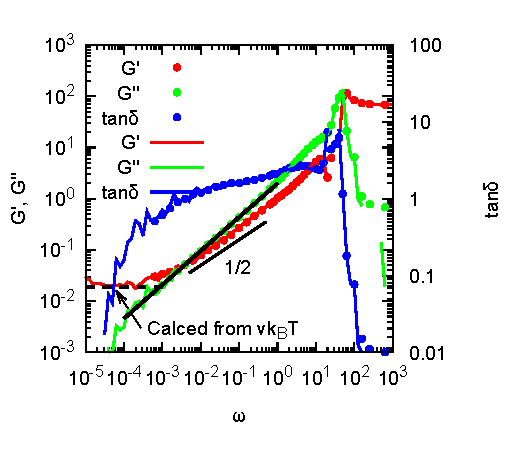
\includegraphics[width=\textwidth]{./fig/N_44_Freq_Sweep.pdf}
\end{figure}
\end{columns}
\end{frame}

%%%%%%%%%%%%%%%%%%%%%%
\begin{frame}
\frametitle{規則構造でのアフィン性}

\begin{columns}[totalwidth=\linewidth]
\column{.4\linewidth}

\begin{itemize}
\item
規則構造においては、
結節点の\alert{連結性は等価}
	\begin{itemize}
	\item
	それぞれの結節点のゆらぎも等価
	\item
	結節点は\alert{規則構造の平均位置に拘束}
\end{itemize}
\item
巨視的な変形後
	\begin{itemize}
	\item
	結節点の\alert{平均位置がアフィン移動}
	\item
	ゆらぎの異方性も類似
	\end{itemize}
\item
緩和モードも単純
\end{itemize}

\column{.58\linewidth}
\begin{figure}
\centering
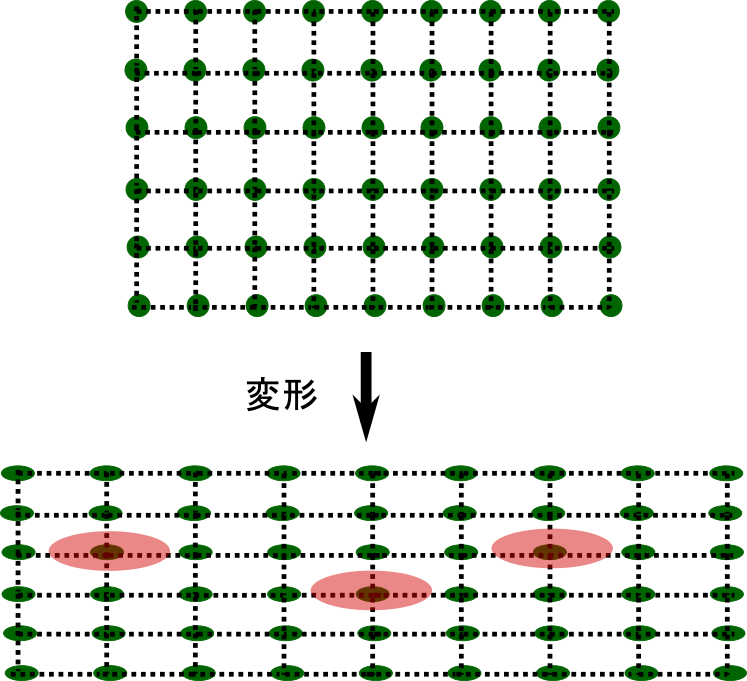
\includegraphics[width=\columnwidth]{./fig/reglar_NW_2.png}
\end{figure}
\end{columns}

\end{frame}
%%%%%%%%%%%%%%%%%%%%%


%%%%%%%%%%%%%%%%
\begin{frame}
\frametitle{す拔け鎖での4分岐規則構造モデル}
\vspace{-3mm}

\begin{columns}[totalwidth=\linewidth]
\column{.48\linewidth}
\begin{block}{検討対象}
\begin{itemize}
\item
ダイヤモンドネットワーク
\item
ストランド
	\begin{itemize}
	\item 
	素抜け鎖
 	\item 
 	ボンド:ハーモニック
 	\item
 	セグメント数 N = 50
 	\item
	システムサイズ\\
	$5\times 5\times 5$
	\end{itemize}
\end{itemize}
\end{block}

\column{.48\linewidth}
\begin{figure}
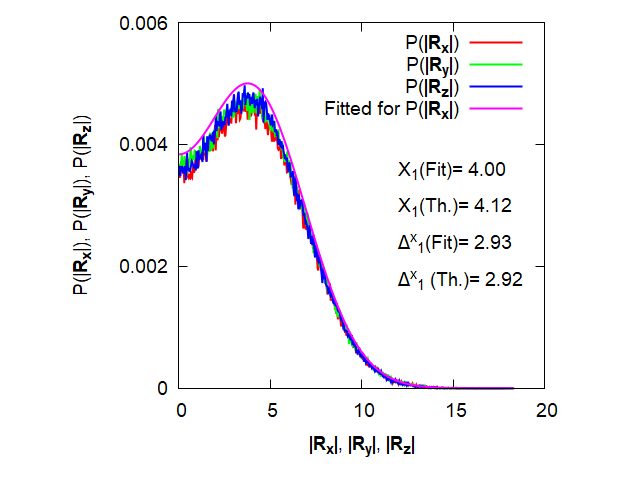
\includegraphics[width=\columnwidth]{./fig/Strand_histgram_reg_4.png}
\end{figure}
\end{columns}

\begin{columns}[totalwidth=\linewidth]
\column{.7\linewidth}
\vspace{-2mm}
\begin{exampleblock}{ストランド長の分布関数}
\begin{itemize}
\item
末端間距離は非ガウス分布
\item
ゆらぎは、理論通りに生じている。
\item
末端間距離が、ほぼ設定通り($|\bm{R_x}| = 4.0$)
\end{itemize}
\end{exampleblock}

\column{.3\linewidth}
\begin{figure}
\centering
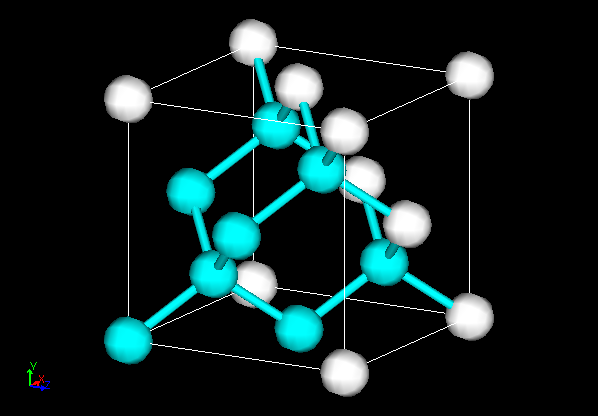
\includegraphics[width=0.8\textwidth]{./fig/dia.png}
\end{figure}

\end{columns}

\end{frame}


%%%%%%%%%%%%%%%%
\begin{frame}
\frametitle{す拔け鎖での4分岐規則構造モデル}
\vspace{-3mm}
\begin{columns}[totalwidth=\linewidth]
\column{.48\linewidth}
\begin{block}{検討対象}
\begin{itemize}
\item
ダイヤモンドネットワーク
\item
ストランド
	\begin{itemize}
	\item 
	素抜け鎖
 	\item 
 	ボンド:ハーモニック
 	\item
 	セグメント数 N = 50
 	\item
	システムサイズ\\
	$5\times 5\times 5$
	\end{itemize}
\end{itemize}
\end{block}

\column{.48\linewidth}
\begin{figure}
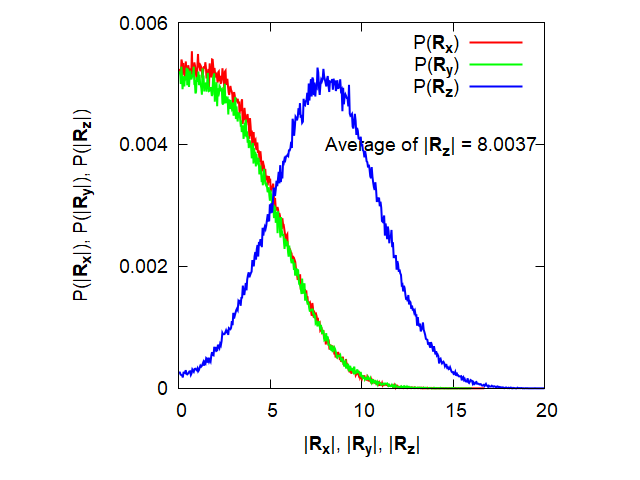
\includegraphics[width=\columnwidth]{./fig/step_4_reg_Strand_histgram.png}
\end{figure}
\end{columns}

\vspace{-2mm}
\begin{exampleblock}{ストランド長の分布関数}
\begin{itemize}
\item
Z軸方向に二倍に伸長
\item
末端間距離は非ガウス分布
\item
伸長方向の末端間距離が、ほぼ二倍に伸長(アフィン変形)\\ $|\bm{R_z}| : 4.0 \Rightarrow 8.0$
\end{itemize}
\end{exampleblock}
\end{frame}


%%%%%%%%%%%%%%%%%%%%%%
\subsection{本発表の内容}
%%%%%%%%%%%%%%%%%%%%%%
\begin{frame}
\frametitle{本発表の内容}

\large
\begin{alertblock}{これまでの検討で出来ていないこと}
\begin{itemize}
\item
MDシミュレーションでファントムネットワークモデルの構築
\item
その力学的及び緩和挙動の明確化。
\end{itemize}

\end{alertblock}

\vspace{-1mm}
\begin{block}{本発表の内容}
\begin{itemize}
\item
ネットワーク構造の連結性にランダム性を導入
\large
	\begin{itemize}
	\item
	ランダム性導入のアルゴリズムの開発
	\item
	ネットワーク・トポロジーの評価
	\end{itemize}
\item
ランダムネットワークモデルの特徴の検討
\large
	\begin{itemize}
	\item
	ランダム性の導入による違いを評価
	\item
	アフィン変形を抑制?
	\item
	ネットワークの力学的応答、緩和の評価
	\end{itemize}
\end{itemize}
\end{block}
\normalsize
\end{frame}
%%%%%%%%%%%%%%%%%%%%%%%%%%
\section{検討内容}
%%%%%%%%%%%%%%%%%%%%%%%%%%
%%%%%%%%%%%%%%%%%%
\begin{frame}
\LARGE{検討内容}
\end{frame}
\subsection{アプローチ}
%%%%%%%%%%%%%%%%%%%%%%
\begin{frame}
\frametitle{アプローチ}

\begin{columns}[totalwidth=1\textwidth]
\column{.4\textwidth}

\begin{block}{連結の異方性の導入}
\begin{itemize}
\item
結節点の連結性にランダム性を導入
\begin{itemize}
\item
解析を容易にするため、結合数、ストランド長を一定
\item
結節点のゆらぎに位置依存性
\end{itemize}
\item
巨視的な変形後
\begin{itemize}
\item
系中に多様な緩和モード
\item
ファントムネットワークモデルの諸特性の発現?
\end{itemize}
\end{itemize}
\end{block}

\column{.55\textwidth}
\begin{figure}
\centering
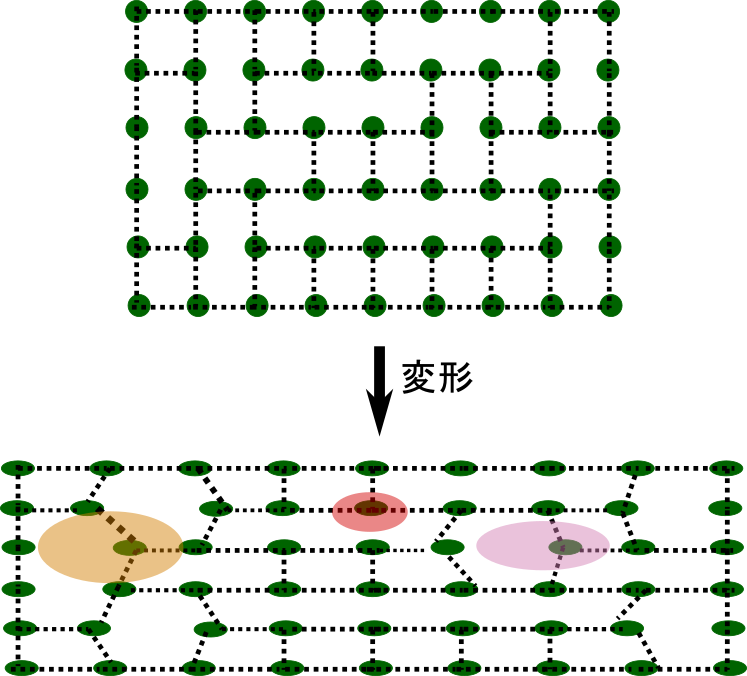
\includegraphics[width=\textwidth]{./fig/連結の異方性_2.png}
\end{figure}

\end{columns}

\end{frame}

%%%%%%%%%%%%%%%%%%%%%%%%%%


%%%%%%%%%%%%%%%%%%%%%%%%%%%%%%%%%
\subsection{ランダムネットワーク構造の作成}
%%%%%%%%%%%%%%%%%%%%%%%%%%
\begin{frame}
\frametitle{ランダムなネットワークの作成}
\small
\vspace{-2mm}
\begin{block}{ここでのランダムの定義}
\begin{itemize}
\item
ユニットセルの連なりとしてネットワークを考え、
\item
各ユニットセルごとにその内部の接続性をランダムとする。
\item
これは、\alert{各ノードの隣接関係をランダム}にすることに対応。
\end{itemize}
\end{block}
\vspace{-1mm}
\begin{exampleblock}{アルゴリズム}
\begin{enumerate}
\item
初期構造の作成
\vspace{-1mm}
	\begin{itemize}
	\item
	\alert{実空間}で8-Chain Model で初期構造を作成。
	\item
	所望の分岐数に\alert{ランダム}に選択した\alert{結合(エッジ)を除去}
	\item
	除去したジオメトリーに対応した\alert{トポロジーモデル}を作成
	\end{itemize}
\item
ランダム性の導入
\vspace{-2mm}
	\begin{itemize}
 	\item 
 	ラプラシアン行列で\alert{全体の連結性を確認}しながら、
 	\item
 	エッジ交換して、ランダム性を導入
	\end{itemize}	
\item
トポロジーモデルに対応する実空間でのネットワーク初期構造作成
\end{enumerate}
\end{exampleblock}
\end{frame}

%%%%%%%%%%%%%%%%%%%%%%%%%%
\begin{frame}
\frametitle{トポロジーモデルへの変換}
\begin{columns}[totalwidth=1\textwidth]
\column{.48\textwidth}
\begin{block}{実空間での初期構造}
\small
\begin{itemize}
\item
$2\times2\times2$ 個のユニットセル
\vspace{-2mm}
\begin{figure}
\centering
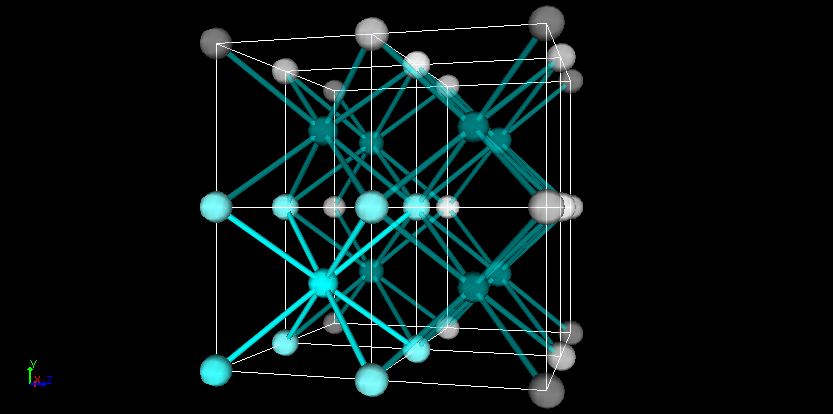
\includegraphics[width=0.8\columnwidth]{./fig/8_per.png}
\end{figure}
\vspace{-2mm}
\item
\vspace{-2mm}
ユニットセルから除去
\vspace{-2mm}
\begin{figure}
\centering
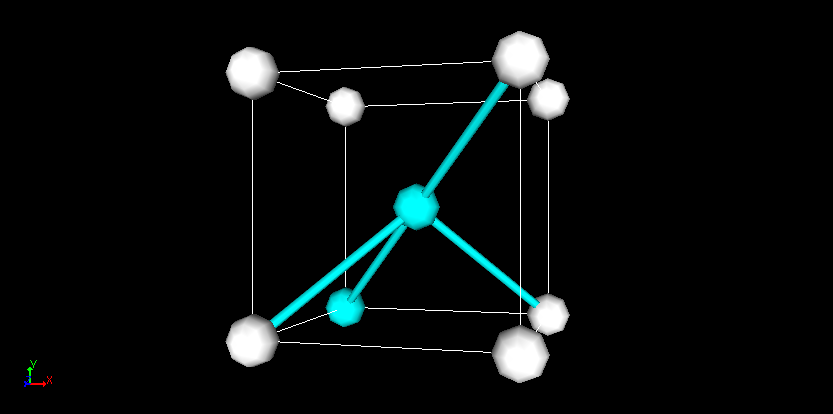
\includegraphics[width=0.8\columnwidth]{./fig/8_4.png}
\end{figure}
\end{itemize}
\end{block}
\column{.48\textwidth}
\begin{exampleblock}{トポロジーモデル}
\small
分岐数を4に減じたトポロジーモデル
\vspace{-2mm}
\begin{figure}
\centering
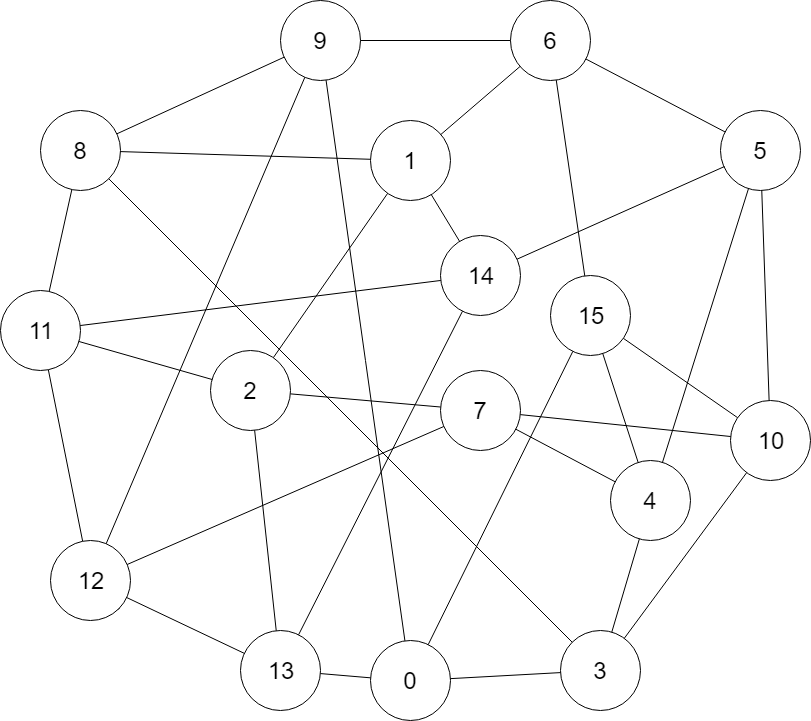
\includegraphics[width=\columnwidth]{./fig/Network.png}
\end{figure}
\end{exampleblock}
\end{columns}
\end{frame}

%%%%%%%%%%%%%%%%%%%%%%%%%%%
\begin{frame}
\frametitle{それぞれの分岐数での初期構造}

\begin{exampleblock}{初期構造の作成}
	\begin{itemize}
	\item
	\alert{実空間}で8-Chain Model で初期構造を作成。
	\item
	所望の分岐数に\alert{ランダム}に選択した\alert{結合(エッジ)を除去}
	\item
	除去したジオメトリーに対応した\alert{トポロジーモデル}を作成
	\end{itemize}
\end{exampleblock}

%\vspace{-3mm}
\begin{columns}[totalwidth=\linewidth]
\column{.45\linewidth}
\begin{block}{検討対象}
\begin{itemize}
\item
分岐数: 3, 4, 5 分岐
\item
3 分岐では、全てが連結していない
\item
4 分岐では、連結していないものもある
\item
5 分岐でも二種類のみ
\end{itemize}
\end{block}
\column{.5\linewidth}
\begin{figure}
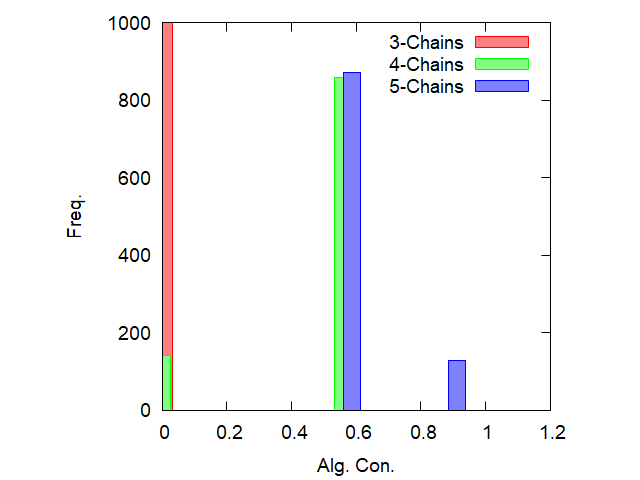
\includegraphics[width=\columnwidth]{./fig/Histgram2.png}
\end{figure}
\end{columns}

\end{frame}

%%%%%%%%%%%%%%%%%%%%%%%%%%
\begin{frame}
\frametitle{トポロジーモデルからのランダム性の導入}

\vspace{-8mm}
\begin{figure}
\centering
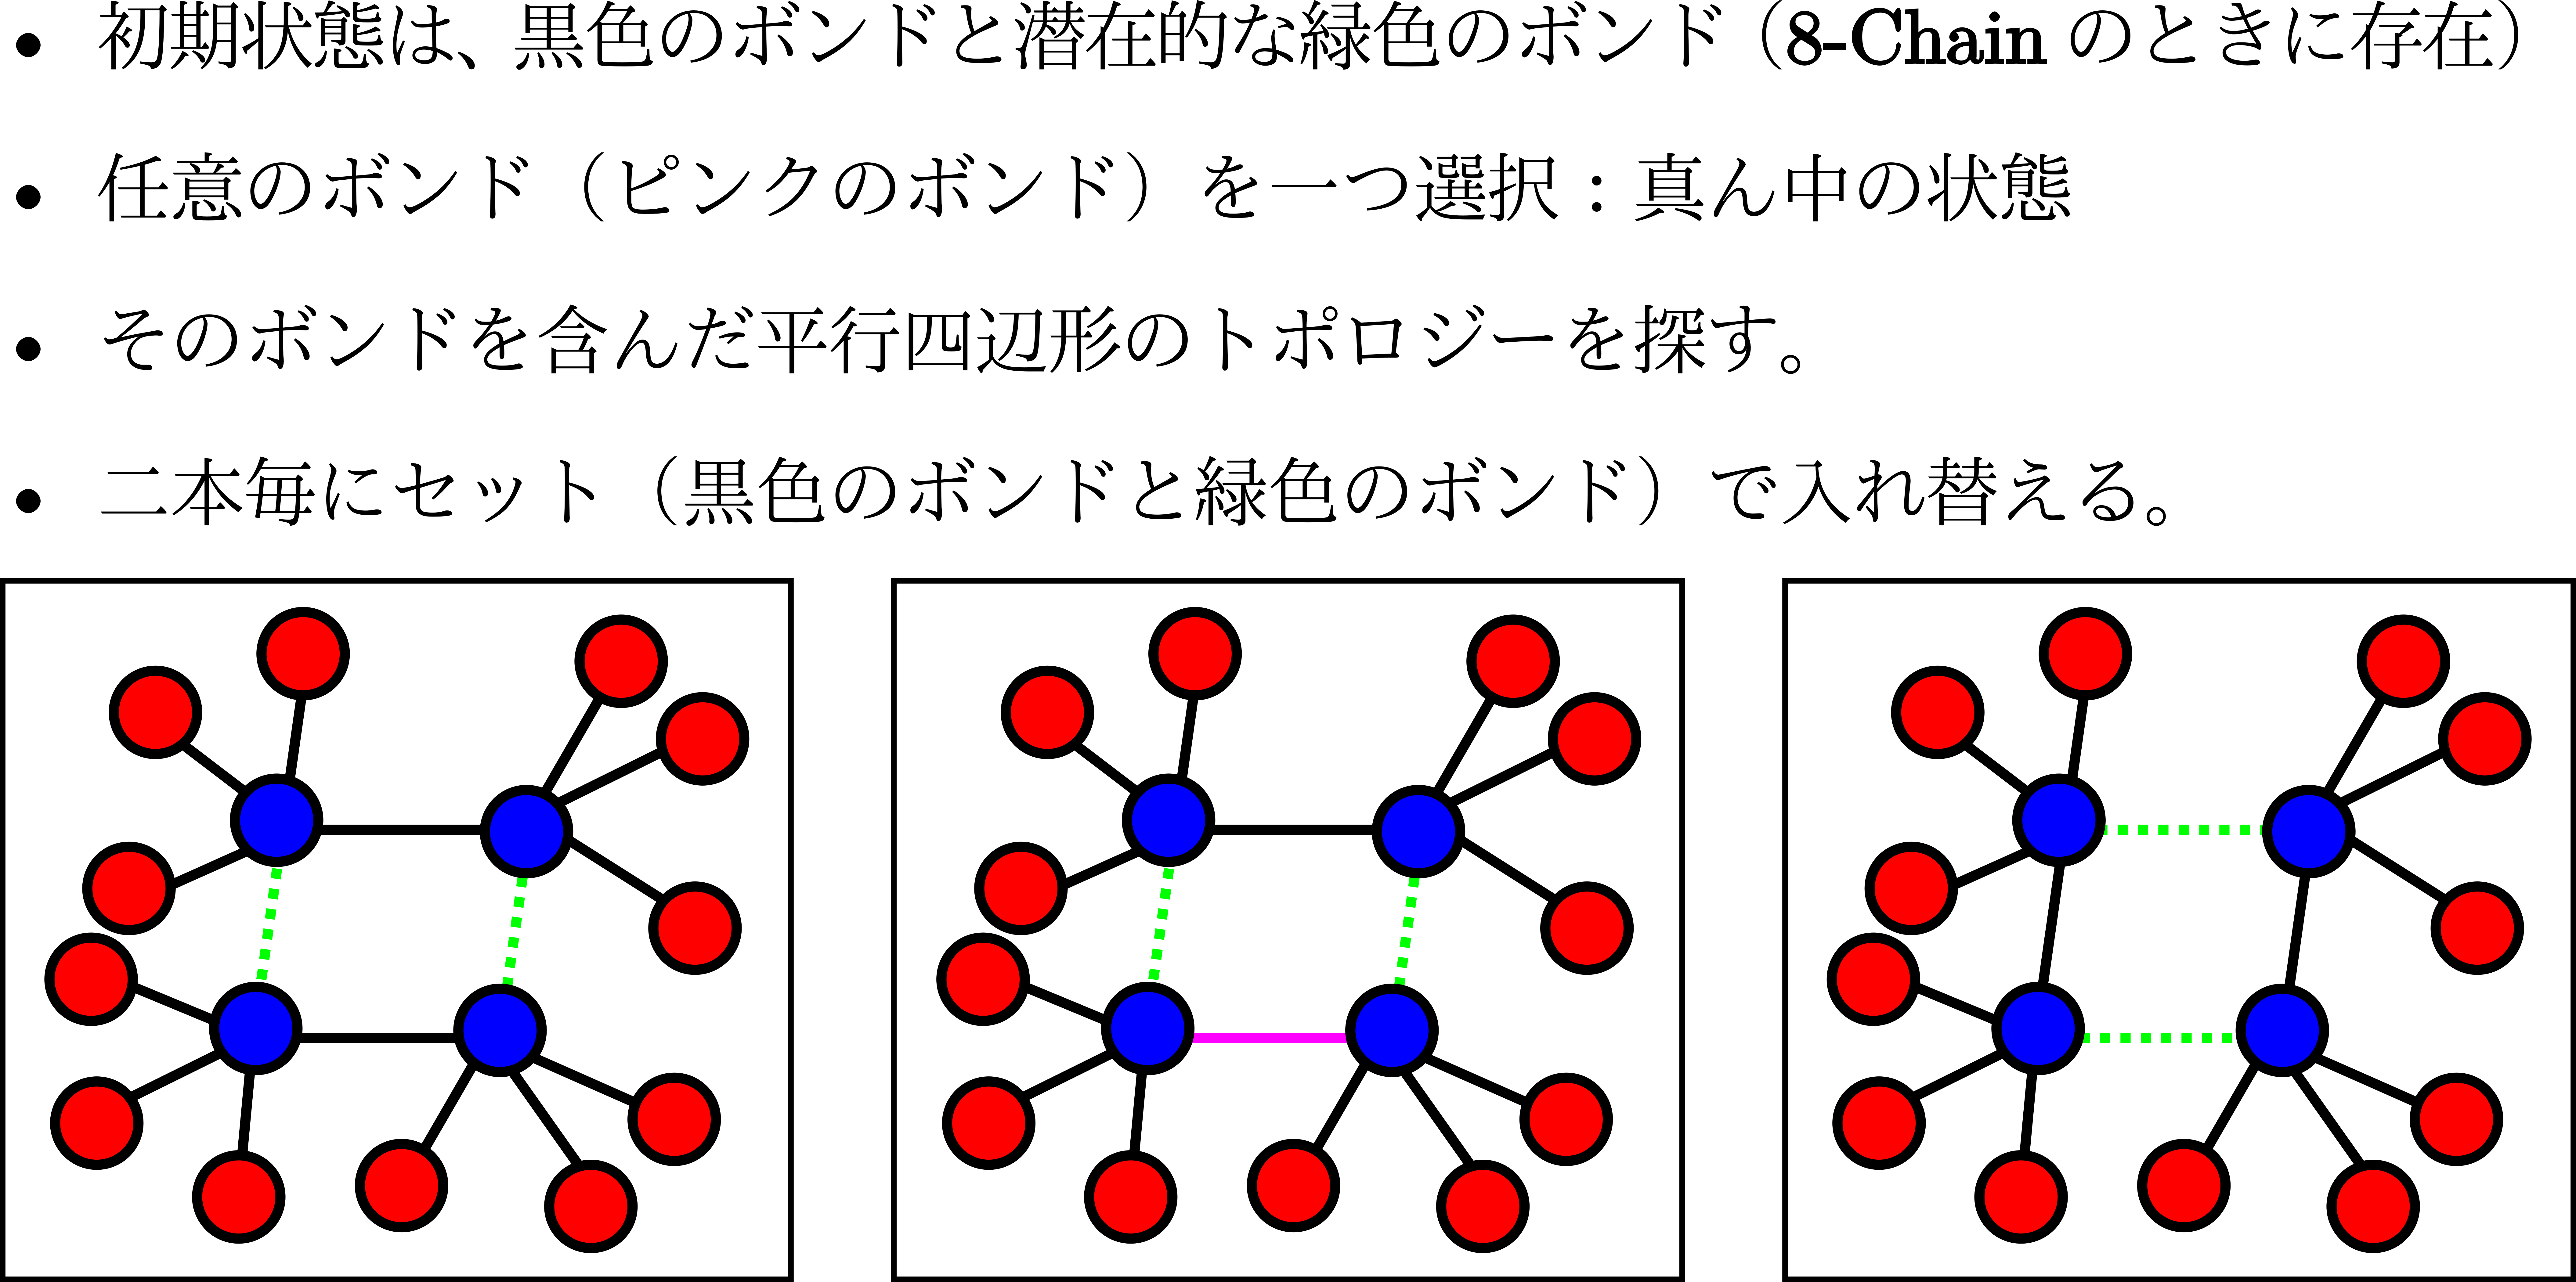
\includegraphics[width=11cm]{./fig/ボンド交換.png}
\end{figure}
\end{frame}

%%%%%%%%%%%%%%%%%%%%%%%%%%
\begin{frame}
\frametitle{$5\times5\times5$ 個のユニットセルでの代数的連結性の分布関数}

\begin{exampleblock}{ボンド交換でのサンプリング数が少ない場合}
\begin{itemize}
\item
3分岐トポロジーモデルは、分布が小さい方に偏在
\item
4分岐のトポロジーモデルでは、二峰性になった。
\end{itemize}
\end{exampleblock}
\vspace{-6mm}
\begin{columns}[totalwidth=1\textwidth]
\column{.5\textwidth}
\begin{figure}
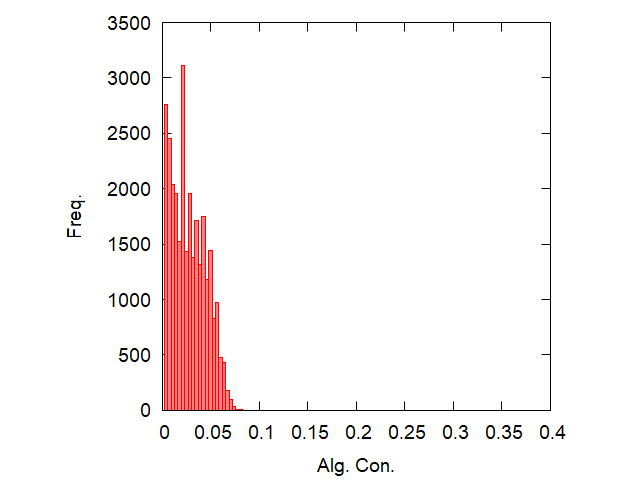
\includegraphics[width=1.1\columnwidth]{./fig/Histgram_3Chain_C5.png}
\end{figure}
\vspace{-3mm}
\centering
\small
3-Chain Model

\column{.5\textwidth}
\begin{figure}
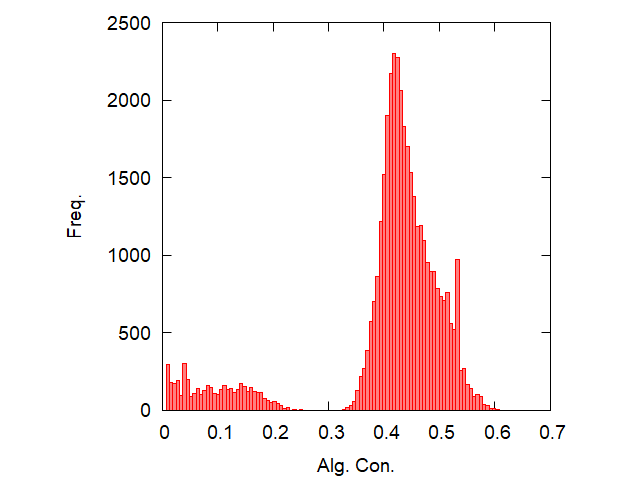
\includegraphics[width=1.1\columnwidth]{./fig/Histgram_4Chain_C5.png}
\end{figure}
\vspace{-2mm}
\centering
\small
4-Chain Model
\normalsize

\end{columns}

\end{frame}

%%%%%%%%%%%%%%%%%%%%%%%%%%
\begin{frame}
\frametitle{代数的連結性の分布関数}

\begin{exampleblock}{サンプリング数の増加($> 1000,000$ times)}
\begin{itemize}
\item
3, 5分岐トポロジーモデルは、単鋒性に
\item
4分岐のトポロジーモデルでは、二峰性\\
サンプリング数を増やすと若干変化
\end{itemize}
\end{exampleblock}

\vspace{-6mm}
\begin{columns}[totalwidth=1\textwidth]
\column{.33\textwidth}
\begin{figure}
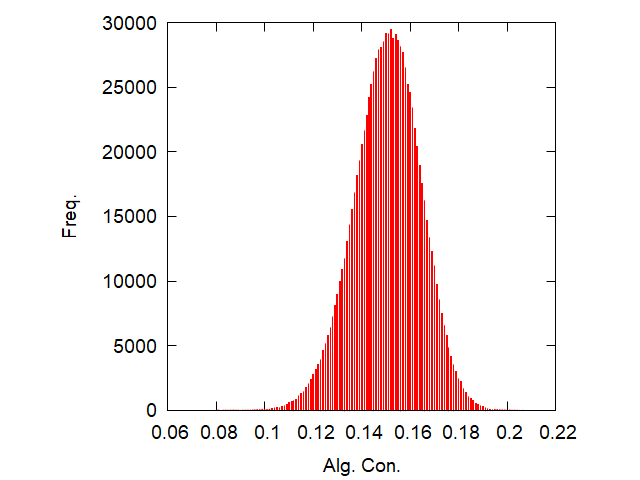
\includegraphics[width=1.2\columnwidth]{./fig/3.png}
\end{figure}
\vspace{-3mm}
\centering
\small
3-Chain Model

\column{.33\textwidth}
\begin{figure}
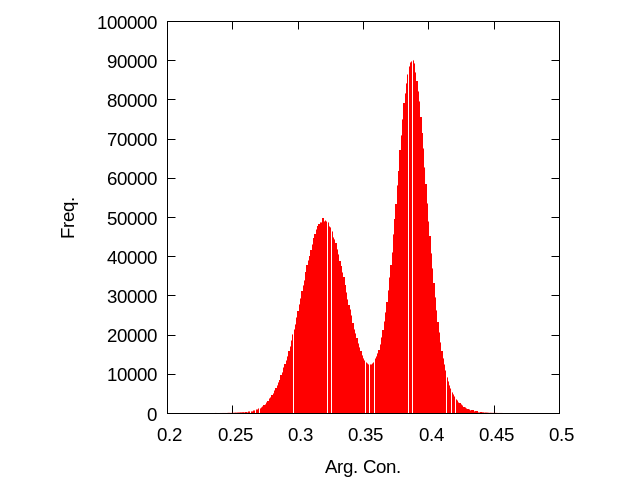
\includegraphics[width=1.2\columnwidth]{./fig/4_1000_5000.png}
\end{figure}
\vspace{-2mm}
\centering
\small
4-Chain Model
\normalsize

\column{.33\textwidth}
\begin{figure}
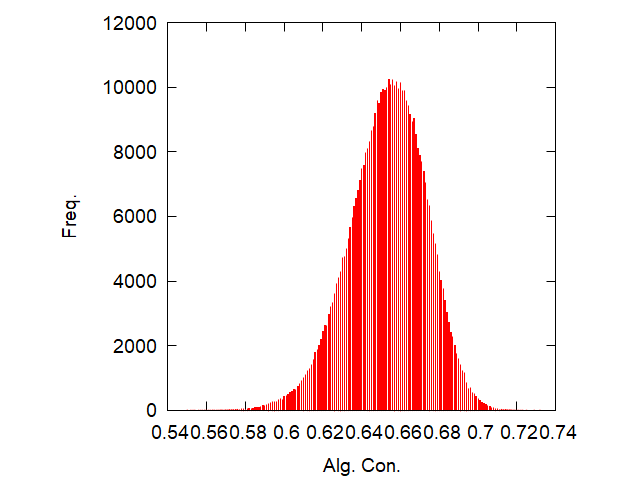
\includegraphics[width=1.2\columnwidth]{./fig/5.png}
\end{figure}
\vspace{-2mm}
\centering
\small
5-Chain Model
\normalsize

\end{columns}

\end{frame}

%%%%%%%%%%%%%%%%%%%
\subsection{四分岐モデルのシミュレーション結果}
%%%%%%%%%%%%%%%%%%%%%%%%%%%
\begin{frame}
\frametitle{四分岐モデルのストランドの末端間距離}

\vspace{-3mm}

\begin{columns}[totalwidth=\linewidth]
\column{.48\linewidth}

\begin{block}{検討対象}
\begin{itemize}
\item
ストランド
	\begin{itemize}
	\item 
	素抜け鎖
 	\item 
 	ボンド:ハーモニック
 	\item
 	セグメント数 N=50 
	\end{itemize}
\item
ランダムネットワーク
	\begin{itemize}
	\item
	四分岐モデル($f=4$)
	\item
	システムサイズ\\
	$5\times 5\times 5$
	\item
	代数的連結性の極大
	\end{itemize}
\end{itemize}
\end{block}

\column{.48\linewidth}
\vspace{-3mm}
\begin{figure}
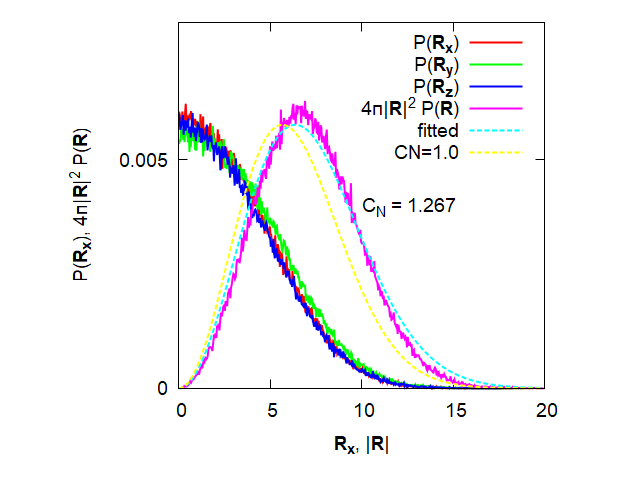
\includegraphics[width=1.2\columnwidth]{./fig/4chain_E2E_init.png}
\end{figure}
\end{columns}

\vspace{-2mm}
\begin{exampleblock}{ストランド長の分布関数}
\begin{itemize}
\item
末端間距離および各方向成分が、ほぼガウス分布
\item
鎖長ゆらぎは、想定されたものよりも若干小さい
\item
末端間距離が設定よりも長く(約 1.3 倍)なっている
\end{itemize}
\end{exampleblock}

\end{frame}

%%%%%%%%%%%%%%%%%%%%%%%%%%%
\begin{frame}
\frametitle{四分岐ランダムネットワークモデルの一軸伸長}
\small
\begin{exampleblock}{一軸伸長:Z軸方向に二倍に伸長}
	\begin{itemize}
	\item
	四分岐ランダムネットワークモデル
	\item
	初期長さ:$|\bm{R_z}| = 3.46$
	\item
	伸長後:$|\bm{R_z}| = 5.62 \Leftarrow$ \alert{二倍には伸びていない}
	\end{itemize}
\end{exampleblock}


\begin{columns}[totalwidth=\linewidth]
\column{.48\linewidth}
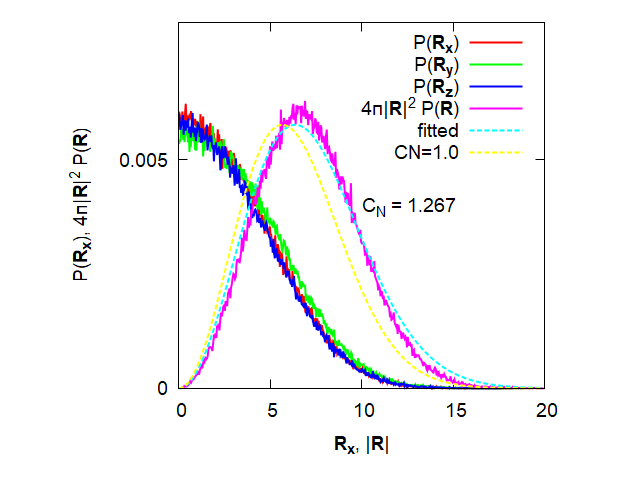
\includegraphics[width=1.1\columnwidth]{./fig/4chain_E2E_init.png}
\column{.48\linewidth}
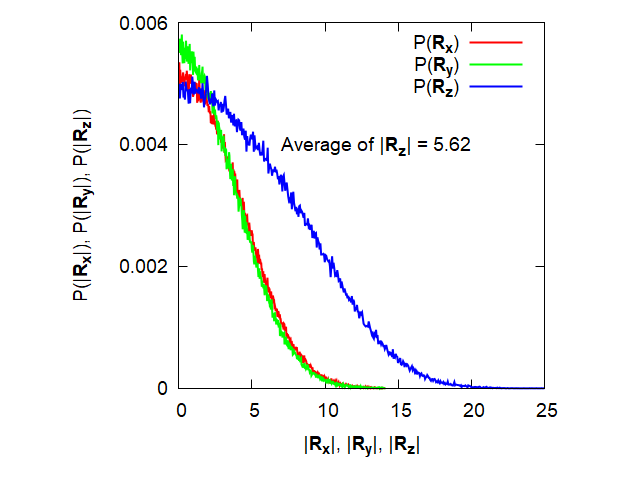
\includegraphics[width=1.1\columnwidth]{./fig/Expand_4_Strand_histgram.png}
\end{columns}

\end{frame}

%%%%%%%%%%%%%%%%%%%%%%%%%%%
\begin{frame}
\frametitle{四分岐ランダムネットワークモデルの一軸伸長}

\vspace{-2mm}
\begin{columns}[totalwidth=\linewidth]

\column{.48\textwidth}
\begin{exampleblock}{内部の鎖が受ける変形}
\begin{itemize}
\item
システム内部の鎖の末端はガウス分布
\item
壁面に固定された末端からの変形が内部に伝達して、
\end{itemize}
\vspace{-5mm}
\tiny
\begin{align*}
&G=\xi \nu k_BT \\
&\begin{cases}
\xi_{\infty} = 1-\dfrac{2}{f} \;\; \text{System}\sim \infty \\[8pt]
\xi_{s} = \dfrac{f-1}{f+1} \;\; \text{Small Limit}
\end{cases}
\end{align*}
\vspace{-7mm}
\begin{figure}
\centering
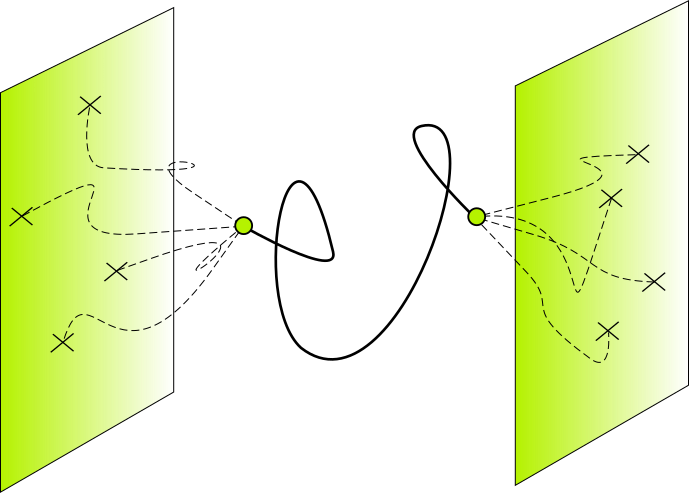
\includegraphics[width=0.6\textwidth]{./fig/phantom.png}
\end{figure}
\end{exampleblock}

\column{.48\linewidth}
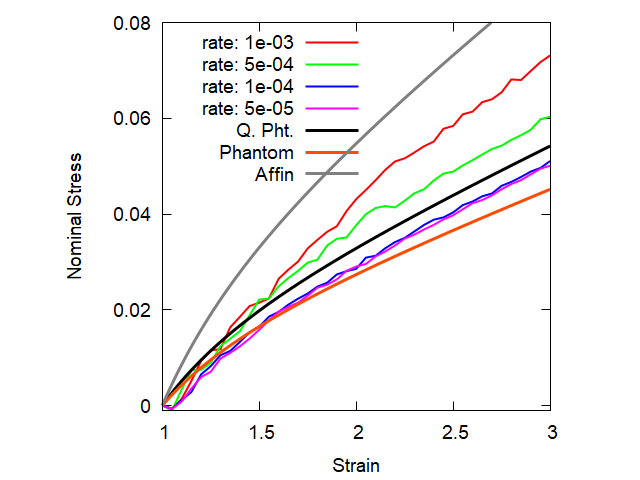
\includegraphics[width=1.2\columnwidth]{./fig/4_ChainSS_multi.png}

\begin{block}{伸長速度依存性}
	\begin{itemize}
	\item
	伸長速度の低下により、
		\begin{itemize}
		\item
		$\xi_{\infty}$ に漸近
		\item
		システムサイズ効果?
		\end{itemize}
	\end{itemize}
\end{block}

\end{columns}

\end{frame}

%%%%%%%%%%%%%%%%%%%%%%%%%%%
\begin{frame}
\frametitle{四分岐ランダムネットワークモデルの応力緩和}
\small

\begin{exampleblock}{高速変形からの応力緩和}
	\begin{itemize}
	\item
	高速変形条件
		\begin{itemize}
		\item
		高速伸長:$\dot{\gamma} = 1e^{-3}$
		\item
		変位:$\lambda = 2$
		\end{itemize}
	\end{itemize}
\end{exampleblock}

\begin{columns}[totalwidth=\linewidth]
\column{.48\linewidth}
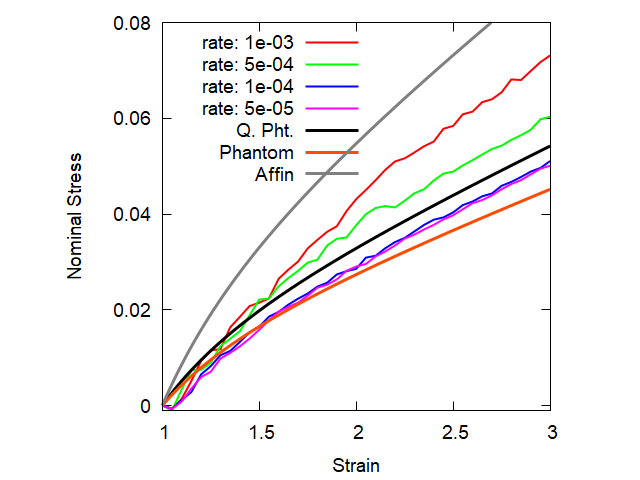
\includegraphics[width=1.2\columnwidth]{./fig/4_ChainSS_multi.png}
\column{.48\linewidth}
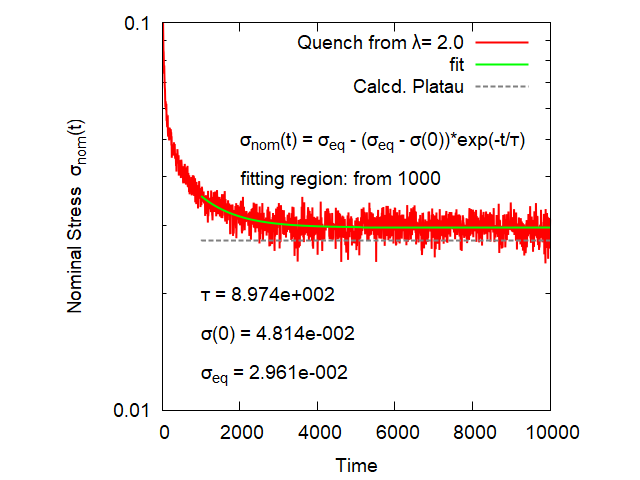
\includegraphics[width=1.2\columnwidth]{./fig/4_Chain_Stress_Quench.png}
\end{columns}

\end{frame}



%%%%%%%%%%%%%%%%%%%%%%%%%%%
\begin{frame}
\frametitle{ネットワークの緩和}

\begin{columns}[totalwidth=\linewidth]
\column{.48\linewidth}

\begin{block}{線形粘弾性測定}
	\begin{itemize}
	\item
	周波数分散測定
	\item
	変形モード
		\begin{itemize}
		\item
		ずり変形
		\item
		Lees-Edward 境界条件
		\item
		歪:$\lambda = 0.1$
		\end{itemize}
	\end{itemize}
\end{block}

\begin{exampleblock}{測定結果}
	\begin{itemize}
	\item
	ランダムネットワークの長時間領域に緩和が見られた
	\item
	結節点のゆらぎに起因する可能性?
	\end{itemize}
\end{exampleblock}

\column{.48\linewidth}
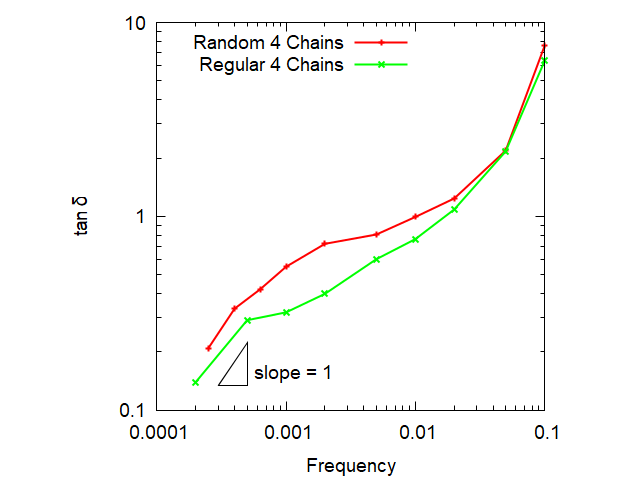
\includegraphics[width=1.3\columnwidth]{./fig/Freq_sweep_tand.png}

\end{columns}

\end{frame}

%%%%%%%%%%%%%%%%%%
\section{おわりに}
%%%%%%%%%%%%%%%%%%
\begin{frame}
\frametitle{おわりに}
\vspace{-2mm}
\begin{block}{本発表の内容}
\begin{itemize}
\item
ネットワーク構造の連結性にランダム性を導入
\large
	\begin{itemize}
	\item
	ランダム性導入のアルゴリズムの開発
	\item
	ネットワーク・トポロジーの評価
	\end{itemize}
\item
ランダムネットワークモデルの特徴の検討
\large
	\begin{itemize}
	\item
	ランダム性の導入による違いを評価
	\item
	ネットワークの力学的応答、緩和の評価
	\end{itemize}
\end{itemize}
\end{block}

\begin{alertblock}{ランダムネットワーク構造のMDシミュレーション}
\begin{itemize}
\item
各ノードごとにランダムな結合性を導入
	\begin{itemize}
	\item
	ストランド長がガウス分布するランダムネットワーク構造
	\end{itemize}
\item
ランダムネットワーク構造の力学的応答
	\begin{itemize}
	\item
	ストランドの変形がノン・アフィン
	\item
	ファントムネットワークモデルの挙動を確認
	\item 
	比較的長時間での緩和を確認
	\end{itemize}
\end{itemize}
\end{alertblock}

\end{frame}


%%%%%%%%%%%%%%%%%%%%%%%%%%%%%%%%%%%%%%%%%%%%%%%
\appendix
%%%%%%%%%%%%%%%%
\begin{frame}
\LARGE{補足資料}
\end{frame}
%%%%%%%%%%%%%%%

%%%%%%%%%%%%%%%%%%%%%%%%%%%%%%
\section{ネットワークのトポロジー}
\subsection{ネットワークのトポロジー}

%%%%%%%%%%%%%%%%%%%%%%%%%%
\begin{frame}
\frametitle{ネットワークの分岐数の処理}
以下のようにノード番号を付与したネットワークを考えると、
\begin{center}
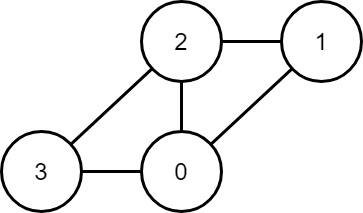
\includegraphics[width=4cm]{./fig/NW-4.png}
\end{center}
隣接行列、および、次数行列は、
\begin{align*}
A = \left( 
\begin{array}{cccc} 
0 & 1 & 1 & 1 \\ 
1 & 0 & 1 & 0 \\
1 & 1 & 0 & 1 \\
1 & 0 & 1 & 0 
\end{array} 
\right) 
,
D = \left( 
\begin{array}{cccc} 
3 & 0 & 0 & 0 \\ 
0 & 2 & 0 & 0 \\
0 & 0 & 3 & 0 \\
0 & 0 & 0 & 2 
\end{array} 
\right) 
\end{align*}
となる。
\end{frame}
%%%%%%%%%%%%%%%%%%%%%%%%%%
\subsection{ラプラシアン行列}
%%%%%%%%%%%%%%%%%%%%%%%%%%
\begin{frame}
\frametitle{ラプラシアン行列}
\begin{columns}[totalwidth=1\textwidth]
\column{.48\textwidth}
ラプラシアン行列は、隣接行列$A$と次数行列$D$により以下のように定義される。
$$
L \equiv D-A
$$
4つのノードからなるネットワークの例であれば、
$$
L = \left( 
\begin{array}{cccc} 
 3 & -1 & -1 & -1 \\ 
-1 &  2 & -1 & 0 \\
-1 & -1 &  3 & -1 \\
-1 &  0 & -1 & 2 
\end{array} 
\right) 
$$
となり、非負の固有値を有する。
\column{.48\textwidth}
グラフが非連結であるとき、%ラプラシアン行列の成分を
連結した成分ごとにブロック対角化できるので、固有値 0 の重複数がグラフの連結成分ブロックの総数となる。
\begin{block}{「代数的連結性」}
「グラフが連結である場合、ラプラシアン行列の固有値 0 の重複数は 1」となる。\\
固有値を昇順にみた時、0 に次ぐ二番目の固有値がグラフの連結性の強さを示す指標となり、「代数的連結性」と呼ばれる。
\end{block}
\end{columns}
\end{frame}
%%%%%%%%%%%%%%%%%%%%%%%%%%%%%%%%%%%%%%%%%%%%%%%%


%%%%%%%%%%%%%%%%%%%%%%%%%%%%%%%%%%%%%%
\section{ファントムネットワークの理論}
%%%%%%%%%%%%%%%%%%%%%%%%%%%%%%%%%%%%%%
\subsection{ファントムネットワークの理論}
%%%%%%%%%%%%%%%%%%%%%%%%%%
\begin{frame}
\frametitle{ファントムネットワークモデルの有限サイズ効果}
\begin{columns}[totalwidth=1\textwidth]
\column{.48\textwidth}
\begin{block}{壁面に末端が固定された効果}
\begin{itemize}
\item
壁面に末端が固定
	\begin{itemize}
	\item  
	$n$ 本のストランド
	\item
	セグメント数: $N$
	\item
	他端が架橋点(位置$\bm{r}$)
	\end{itemize}
\item
架橋点の運動性
	\begin{itemize}
	\item  
	壁と$N/n$ 個の短いストランドと等価
	\item
	壁の移動(変形)の影響減少
	\end{itemize}
\end{itemize}
\vspace{-2mm}
\begin{figure}
\centering
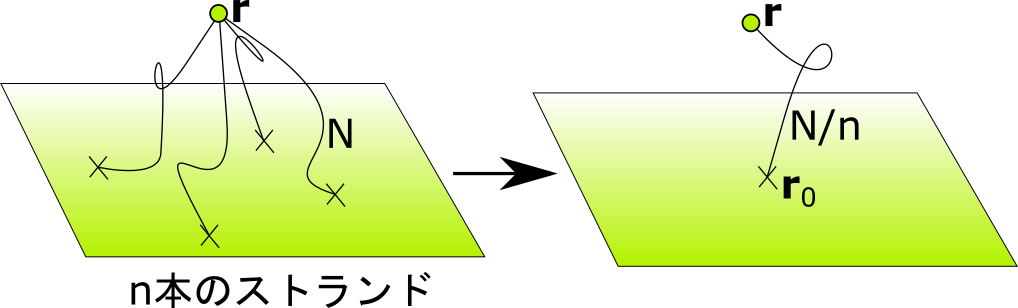
\includegraphics[width=\textwidth]{./fig/phantom-1.png}
\end{figure}
\end{block}
\column{.48\textwidth}
\begin{exampleblock}{内部の鎖が受ける変形}
\begin{itemize}
\item
システム内部の鎖の末端はガウス分布
\item
壁面に固定された末端からの変形が内部に伝達して、
\end{itemize}
\vspace{-5mm}
\tiny
\begin{align*}
&G=\xi \nu k_BT \\
&\begin{cases}
\xi_{\infty} = 1-\dfrac{2}{f} \;\; \text{System}\sim \infty \\[8pt]
\xi_{s} = \dfrac{f-1}{f+1} \;\; \text{Small Limit}
\end{cases}
\end{align*}
\vspace{-7mm}
\begin{figure}
\centering
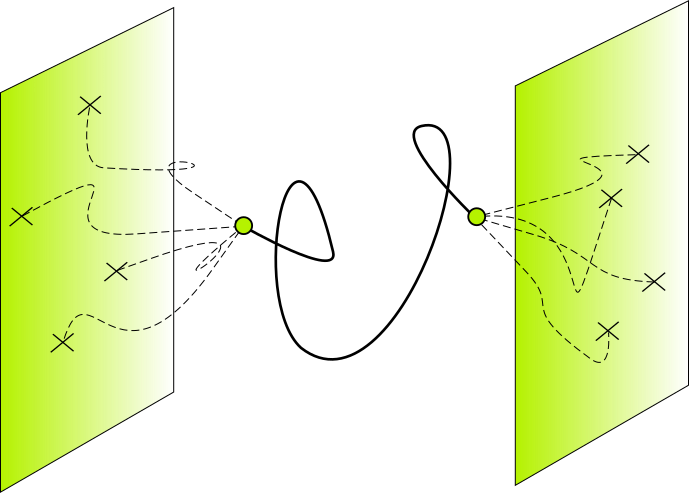
\includegraphics[width=0.6\textwidth]{./fig/phantom.png}
\end{figure}
\end{exampleblock}
\end{columns}
\end{frame}
%%%%%%%%%%%%%%%%%%%%%%%%%%

%%%%%%%%%%%%%%%%%%%%%%%%%%%%%%%%%%%%%%%%%%%%%%
\subsection{ファントムネットワークの振る舞い}
%%%%%%%%%%%%%%%%%%%%%%%%%%%%%%%%%%%%%%%%%%%%%%
\begin{frame}
\frametitle{ファントムネットワークのゆらぎ}

\begin{columns}[totalwidth=1\textwidth]
\column{.47\textwidth}
\scriptsize
\begin{block}{ゆらぎの入ったポテンシャル}
ストランドの末端間ベクトル $\bm{R}_{nm}$ を、\\架橋点の位置ベクトル $\bm{r}_n$ を用いて、
\vspace{-3mm}
\begin{equation*}
\bm{R}_{nm} \equiv \bm{r}_n-\bm{r}_m
\end{equation*}

系のポテンシャルエネルギーは、
\vspace{-3mm}
\begin{equation*}
U=\dfrac{k}{2} \sum_{\langle nm \rangle} \bm{R}_{nm}^2
\end{equation*}

これは、自然長で決まる定数項と、ゆらぎに起因した第二項に分割でき、その和で以下となる。
\vspace{-3mm}
\begin{equation*}
U=\dfrac{k}{2} \sum_{\langle nm \rangle} {\bm{R}_{nm}^{(0)}}^2 + \dfrac{k}{2} \sum_{\langle nm \rangle} \Delta \bm{R}_{nm}^2
\end{equation*}
\end{block}

\column{.47\textwidth}
\scriptsize
\begin{block}{アンサンブル平均の二つの表式}
\vspace{-5mm}
\begin{align*}
 \begin{cases}
	\langle U \rangle = N_{strands} \dfrac{k}{2} \langle \Delta \bm{R}^2 \rangle \\
	\langle U \rangle = 3(N_{nodes}-1) \dfrac{1}{2} k_B T
 \end{cases}
\end{align*}
なお、第二式は等分配側より導出した。
\end{block}

\begin{exampleblock}{ファントムネットワークでのゆらぎ}
架橋点数 $N_{nodes}$、架橋点官能基数 $f$ とすれば、規則格子での一般式として、
\vspace{-3mm}
\begin{equation*}
\langle \Delta \bm{R}^2 \rangle = \dfrac{3k_B T}{k} \dfrac{2}{f} \left( 1-\dfrac{1}{N_{nodes}} \right)
\end{equation*}

適切な条件で、ストランドの自然長 $R_0$\\
を用いて、
\vspace{-3mm}
\begin{equation*}
\color{red}
\langle \Delta \bm{R}^2 \rangle = \dfrac{2}{f} R_0^2
\end{equation*}
\vspace{-6mm}
\end{exampleblock}

\end{columns}

\end{frame}


%%%%%%%%%%%%%%%%%
\begin{frame}
\frametitle{ファントムネットワークの振る舞い}

\begin{columns}[totalwidth=1\textwidth]
\column{.47\textwidth}
\scriptsize
\begin{block}{ストランドの末端間距離}
ストランドの末端間距離の分布関数は、畳み込み積分の形で、
\vspace{-3mm}
\begin{equation*}
\Omega(\bm{R}) = \Phi(\bar{\bm{R}}) + \Psi(\bm{\Delta R})
\end{equation*}

ダイヤモンド構造でのストランド末端間距離の $x$ 成分の分布関数 $P_{strand}(x)$ は、\vspace{-3mm}
\begin{align*}
P_{strand}(x) 
&= \dfrac{1}{2}\dfrac{1}{\sqrt{2\pi}\Delta_{\lambda}^x} \\
&\times \left[ \exp\left(-\dfrac{(x-X_{\lambda})^2}{2(\Delta_{\lambda}^x)^2} \right) \right. \\
&\quad \left. + \exp\left(-\dfrac{(x+X_{\lambda})^2}{2(\Delta_{\lambda}^x)^2} \right) \right]
\end{align*}
なお、$X_{\lambda}$、$\Delta_{\lambda}^x$ は、伸長比 $\lambda$ である時の、ストランド長及びゆらぎの $x$ 成分を表す。
\end{block}

\column{.47\textwidth}
\scriptsize
\begin{block}{ずり弾性率 $G_{ph}$}
ファントムネットワークでのずり弾性率 $G_{ph}$ は、以下の表式で表される。
\vspace{-3mm}
\begin{align*}
G_{ph} &= \dfrac{1}{3} \dfrac{1}{V} \left. \dfrac{d^2 F_{ph}}{d \lambda^2} \right|_{\lambda = 1}\\
&=\dfrac{\langle R_{strand}^2 \rangle}{\langle R_0^2 \rangle} \nu k_B T
\end{align*}
ここで、$\nu$ は、ストランドの数密度である。

\vspace{3mm}
ダイヤモンド構造のように規則構造からなるネットワークにおいて、各ストランド長がガウス鎖の二乗平均末端距離となるようにシステムサイズを設定した場合、$\langle R_{strand}^2 \rangle = \langle R_0^2 \rangle$ であるので、
\vspace{-3mm}
\begin{align*}
\color{red}
G_{ph}= \nu k_B T
\end{align*}

\end{block}
\end{columns}
\end{frame}
%%%%%%%%%%%%%%%%%%%%%%%

%%%%%%%%%%%%%%%%%%%%%%%%%%%%
\section{その他}

\subsection{破壊について}
%%%%%%%%%%%%%%%%%%%%%%%%%%%%

\begin{frame}
\frametitle{高分子材料への期待と不安}
{\Large
地球温暖化対策の CO$_2$ 削減へ向けて、\\
{\color{red}「自動車を中心とした運送機器の抜本的な軽量化」}
\\
が提唱されている。}

\begin{block}{高分子材料への期待}
	\begin{itemize}
	\item
	現行の鉄鋼主体$ \Rightarrow$ 高分子材料を含むマルチマテリアル化
	
	\item
	高分子材料によるマルチマテリアル化のポイント
		\begin{itemize}
		\item
		高い比強度の有効利用
		\item
		特徴を生かした適材適所 $\Leftrightarrow$ 適切な接合方法の選択
			\begin{itemize}
			\large
			\item
			{\color{red} 「接着接合」への高分子の利用}
			\item
			{\color{red} 「柔らかさを生かした弾性接着接合」}
			\end{itemize}
		\Large
		\item
		{\color{blue}耐久性が不明確(特に疲労破壊に対して)}
		\end{itemize}
	\end{itemize}
\end{block}
\normalsize
\end{frame}

%%%%%%%%%%%%%%%%%%%%%%%%%%%%%%
\begin{frame}
\frametitle{破壊工学の考え方}
\begin{exampleblock}{破壊工学の考え方}

\begin{itemize}
\item
系中にクラックが存在することを前提に材料の耐久性を評価
\item
\alert{「クラック近傍での応力集中を如何に抑制するか」}がポイント
\end{itemize}
\end{exampleblock}

\begin{columns}[totalwidth=1\textwidth]
\column{.5\textwidth}
\begin{alertblock}{破壊工学の観点から(微視的)}
	\begin{itemize}
		\item
		クラック先端での応力集中\\ \alert{応力拡大係数 $K_I$ で評価}
		\footnotesize
		\begin{align*}
		K_{I} = \sigma \sqrt{\pi c}
		\end{align*}
		\normalsize
		\item 
		クラック進展の抑制 \\
		$\Rightarrow$ 先端での\alert{局所降伏}\\
		降伏応力 $\sigma_Y$ に反比例
		\footnotesize
		\begin{align*}
		d \propto \left( \dfrac{K_I}{\sigma_Y} \right)^2
		\end{align*}
		\normalsize
	\end{itemize}
\end{alertblock}
\column{.5\textwidth}
	\centering
	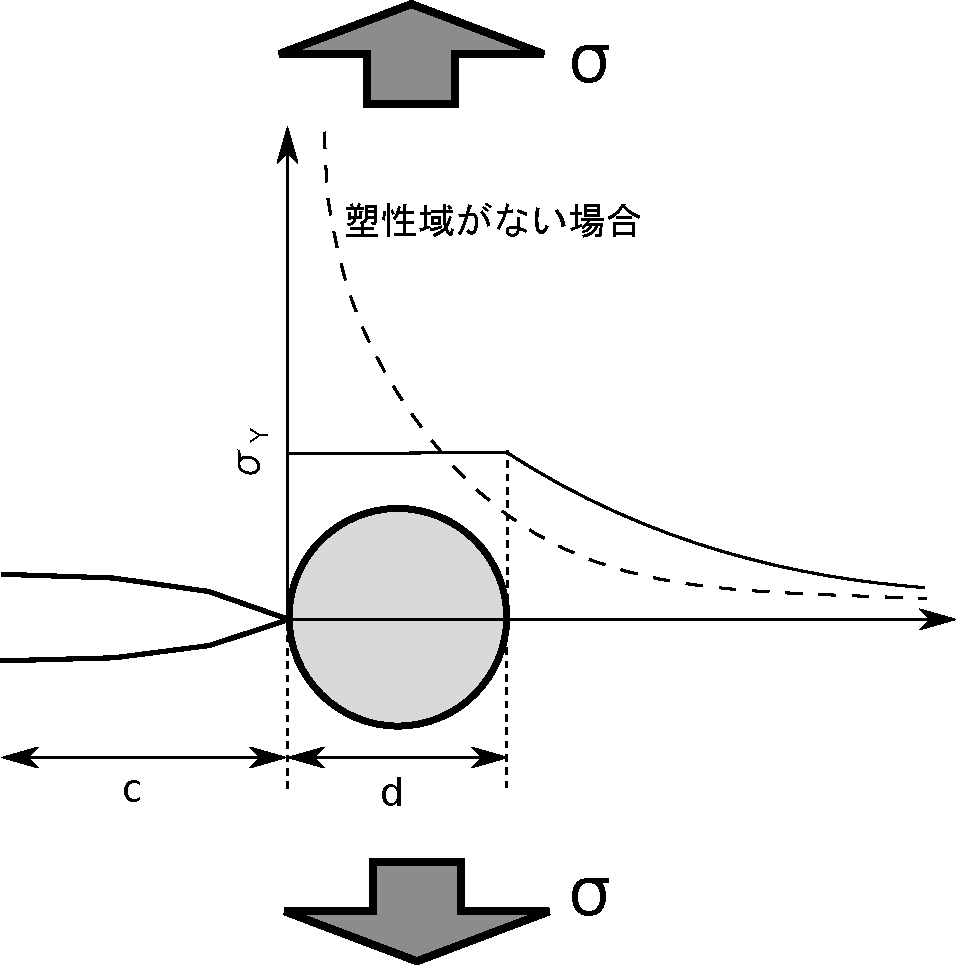
\includegraphics[width=45mm]{./fig/Crack_Yield.pdf}
\end{columns}

\end{frame}

%%%%%%%%%%%%%%%%%%%%%%
\subsection{破壊と粘弾性}
%%%%%%%%%%%%%%%%%%%%%%
\begin{frame}
\frametitle{ゴムの強靭性}


\begin{columns}[totalwidth=1\textwidth]
\column{.6\textwidth}
\begin{exampleblock}{Andrews 理論}
クラック先端の応力の等高線表示
	\begin{itemize}
	\item
	クラック成長時の応力場の考察より、
		\begin{itemize}
		\item
		{\color{red} Loading 場とUnloading 場の差}が重要。
		\item
		この差は\alert{ヒステリシスに由来}
		\end{itemize}	
	\item
	\alert{ひずみエネルギー開放率が低減} \\$\Rightarrow$ 強靭さの起源。
	\end{itemize}
\end{exampleblock}

{Andrews, E. H. and Fukahori, Y., Journal of Materials Science, 12, 1307 (1977)}

\column{.4\textwidth}
\centering
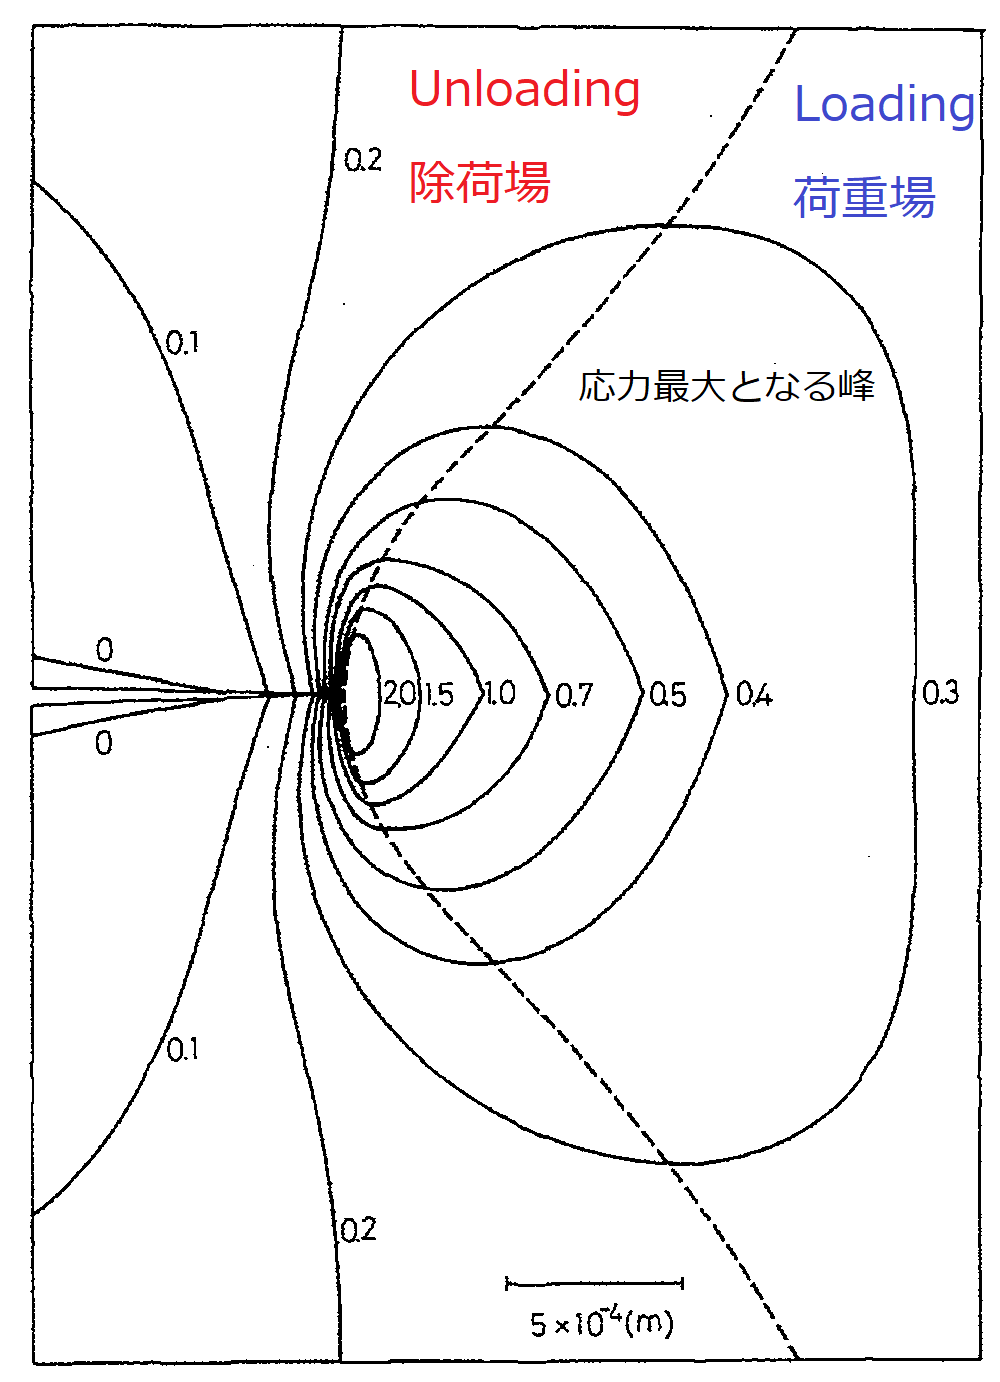
\includegraphics[width=40mm]{./fig/crack.png}
\end{columns}
\end{frame}


%%%%%%%%%%%%%%%%%
\begin{frame}
\frametitle{ゴムの破壊と粘弾性}

\vspace{-2mm}
\begin{alertblock}{ゴムの破壊}
大変形を伴う非線形現象だが、時間温度換算則の成立が多数報告
\end{alertblock}

\begin{columns}[totalwidth=1\textwidth]
\column{.48\textwidth}
ゴムの亀裂先端近傍での大変形
\centering
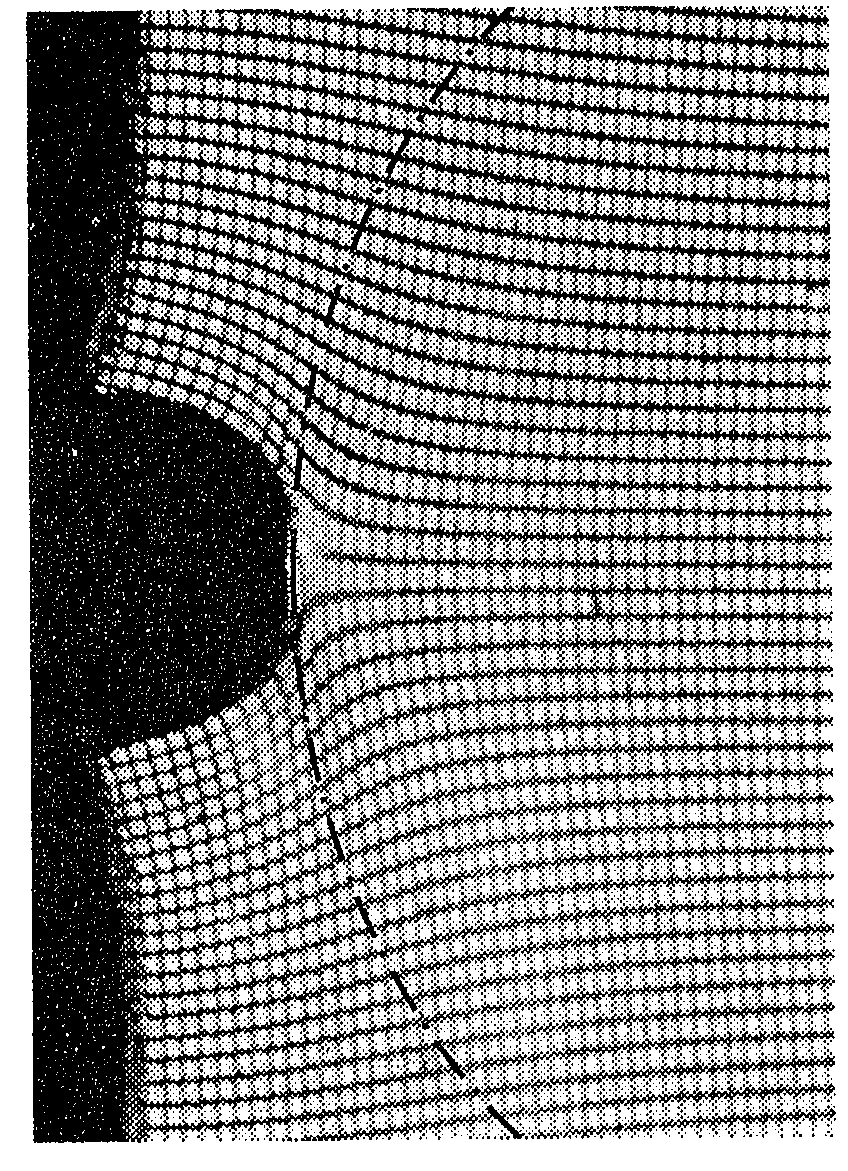
\includegraphics[width=.7\textwidth]{./fig/rubber_crack.png}
\column{.48\textwidth}
時間温度換算則の成立
\centering
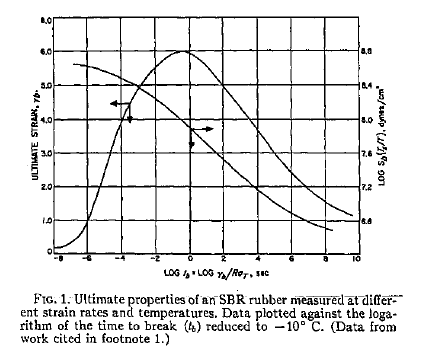
\includegraphics[width=\textwidth]{./fig/Time_Temp_2.png}

{\tiny Smith T., Stedry P., J. Appl. Phys. (1960) 31 1892}

\end{columns}
\end{frame}


%%%%%%%%%%%%%%%%%
\begin{frame}
\frametitle{SBRでの伸びきり効果}

\centering
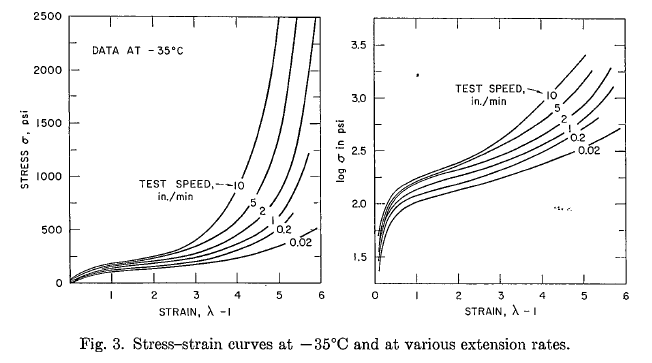
\includegraphics[width=8.5cm]{./fig/SBR_lowTemp_2.png}

{\tiny Smith TL., Dickie RA., J. Pol. Sci. part A-2 (1969) 7 635}

\begin{alertblock}{室温で伸び切りが出ないはずのSBR}
\begin{itemize}
\item
低温、高速変形でSBRでも伸びきり効果が発現
\item
時間温度換算則で考えてみれば?
\end{itemize}
\end{alertblock}
\end{frame}

%%%%%%%%%%%%%%%
\begin{frame}
%[shrink squeeze]
\frametitle{高分子材料の疲労と破壊}
\begin{columns}[totalwidth=1\textwidth]
\column{.6\textwidth}
ガラス状態の高分子材料では、
\begin{block}{破壊のモード(巨視的)}
脆性破壊 $\Leftrightarrow$ 延性破壊\\
脆性破壊は、降伏前にミクロなクラックが進展した破壊とも考えられる。
\end{block}
\column{.4\textwidth}
	\centering
	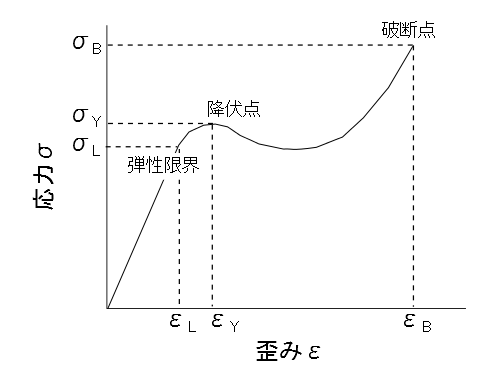
\includegraphics[width=\textwidth]{./fig/S_S_Curve.png}
\end{columns}
\begin{exampleblock}{降伏と劣化}
	\begin{itemize}
	\item
	靭性向上のため
	\begin{itemize}
		\item
		{\color{red} 局所的な降伏}が必須。(クレイズのような局所的な破壊も含む)
		\item 
		一般に、高分子材料の{\color{red} 降伏は不可逆}。
	\end{itemize}
	\item
	降伏による劣化
		\begin{itemize}
			\item 
			降伏 $\Leftrightarrow$ {\color{red} 本質的には、少しずつ破壊。}
			\item
			{\color{red} 破壊領域への水分の浸透 $\Leftarrow$ 長期耐久性の欠如}
		\end{itemize}
	\end{itemize}
\end{exampleblock}
\end{frame}

%%%%%%%%%%%%%%%%%%%%%%%%%%%%
\subsection{ネットワークの振る舞い}
%%%%%%%%%%%%%%%%%%%%%%%%%%%%%%%%%%%%%%%%%%%%%%%%
\begin{frame}
\frametitle{架橋点近傍の拘束状態に基づく二つのモデル}
\begin{columns}[totalwidth=1\textwidth]
\column{.5\textwidth}
ストランドと架橋点の模式図
%\centering
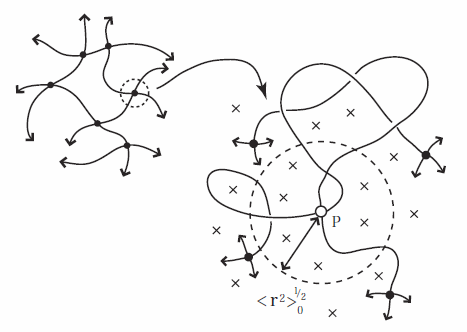
\includegraphics[width=\textwidth]{./fig/JP_vicinity.png}
架橋点はストランド経由で直接連結した架橋点(図中の黒丸)以外の、近接する多数のストランド及び架橋点(図中の×)に囲まれている。
\column{.5\textwidth}
\begin{itemize}
\item
``Affine NW Model''\\
架橋点は周辺に強く拘束され巨視的変形と相似に移動。\\(Affine 変形)
\footnotesize
\begin{equation*}
G=\nu k_B T
\end{equation*}
\normalsize
$\nu$ は、ストランドの数密度
\item
``Phantom NW Model''\\
架橋点が大きく揺らぎ、実効的なずり弾性率($G$)が低下。
\footnotesize
\begin{align*}
G&=\xi \nu k_B T \\
\xi&= 1 -\dfrac{2}{f}
\end{align*}
\normalsize
$f$ は架橋点の分岐数
\end{itemize}
\end{columns}
\end{frame}

%%%%%%%%%%%%%%%%%%%
\begin{frame}
\frametitle{架橋点の近傍}
\centering
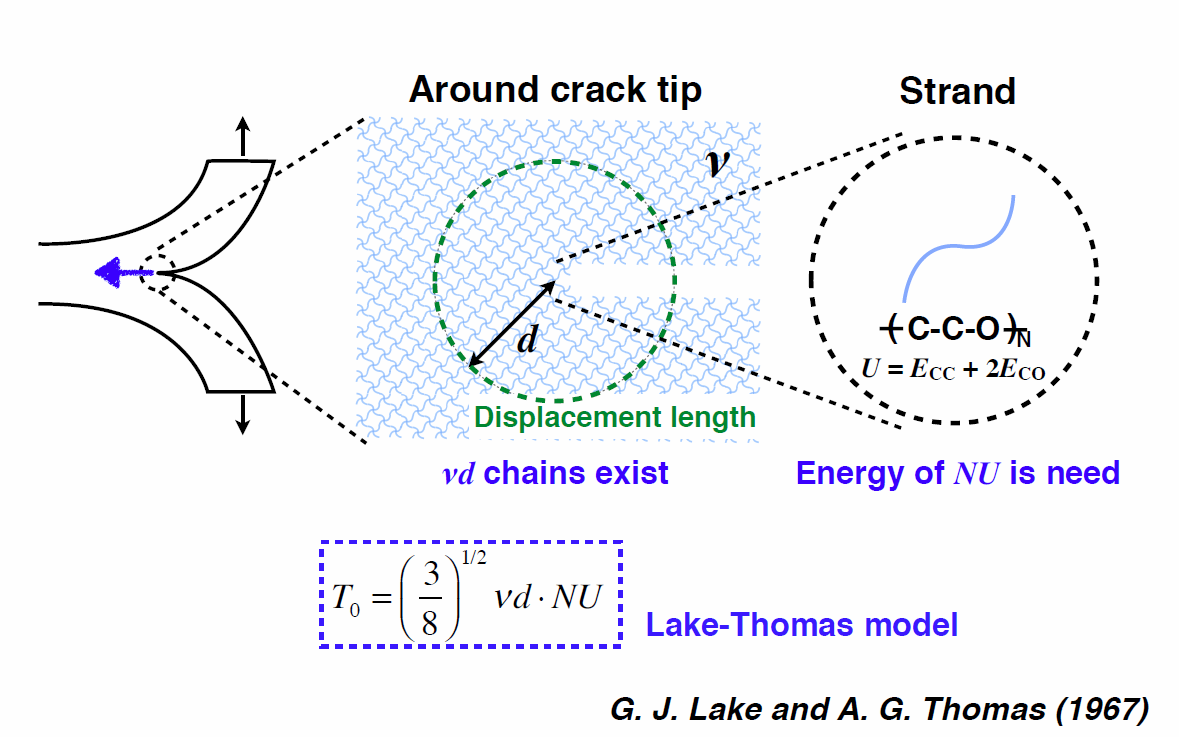
\includegraphics[width=100mm]{./fig/Lake_Thomas.png}
\end{frame}
%%%%%%%%%%%%%%%%%%


\end{document}
